% Grobe  Architekturbeschreibung  durch  Bausteine/Komponenten  (Kein  detailliertes Klassendiagramm).
\section{Systemübersicht}

Dieses Kapitel bietet zunächst eine grobe Übersicht des Systems und der Abgrenzung von Benutzer Algorithmen und Modulen des 3DMuVi-Programms. Außerdem wird die Interaktion der Module durch ein Datenflussdiagramm veranschaulicht. Im Anschluss werden die Anwendungsfälle vorgestellt. Schlussendlich werden Typische Nutzungsabläufe vorgestellt die die Software umsetzen muss. Diese werden jeweils mit einem  Sequenzdiagramm visualisiert.
\subsection{Architektur}

Aufgrund der Komplexität und Größe, wird das 3DMuVi-Programm nicht durch ein einzelnes Entwurfsmuster wie beispielsweise Model-View-Controller (MVC) umgesetzt. Stattdessen wird es zunächst in einzelne Module aufgeteilt.
Durch die einzelnen Module, die aufgabenspezifisch getrennt werden, wird eine bessere Übersicht und Struktur des Programms gewährleistet. Außerdem kann der Arbeitsaufwand somit effektiver aufgeteilt werden.\newline
Die einzelnen Module werden im Entwurf weiter aufgeteilt. Nach Möglichkeit wird das Entwurfsmuster MVC verwendet.\newline Da 3DMuVi nur ein Framework anbietet, werden zusätzliche Algorithmen benötigt.
Die benötigten Algorithmen werden durch eine Plugin-Struktur an das Programm gegeben.\newline \newline
Es wird in folgende 6 Module aufgeteilt:
\begin{itemize}
\item Workflow
\item I/O
\item Visualisierung
\item Logger
\item Einstellungen
\item Interaktion
\end{itemize}

\subsection{Übersicht}
Im Folgenden Diagramm wird die Abgrenzung von 3DMuVi, Benutzer und Algorithmen veranschaulicht.
Der Benutzer liefert die Algorithmen und interagiert jeweils mit den Schnittstellen der einzelnen Modulen.\newline
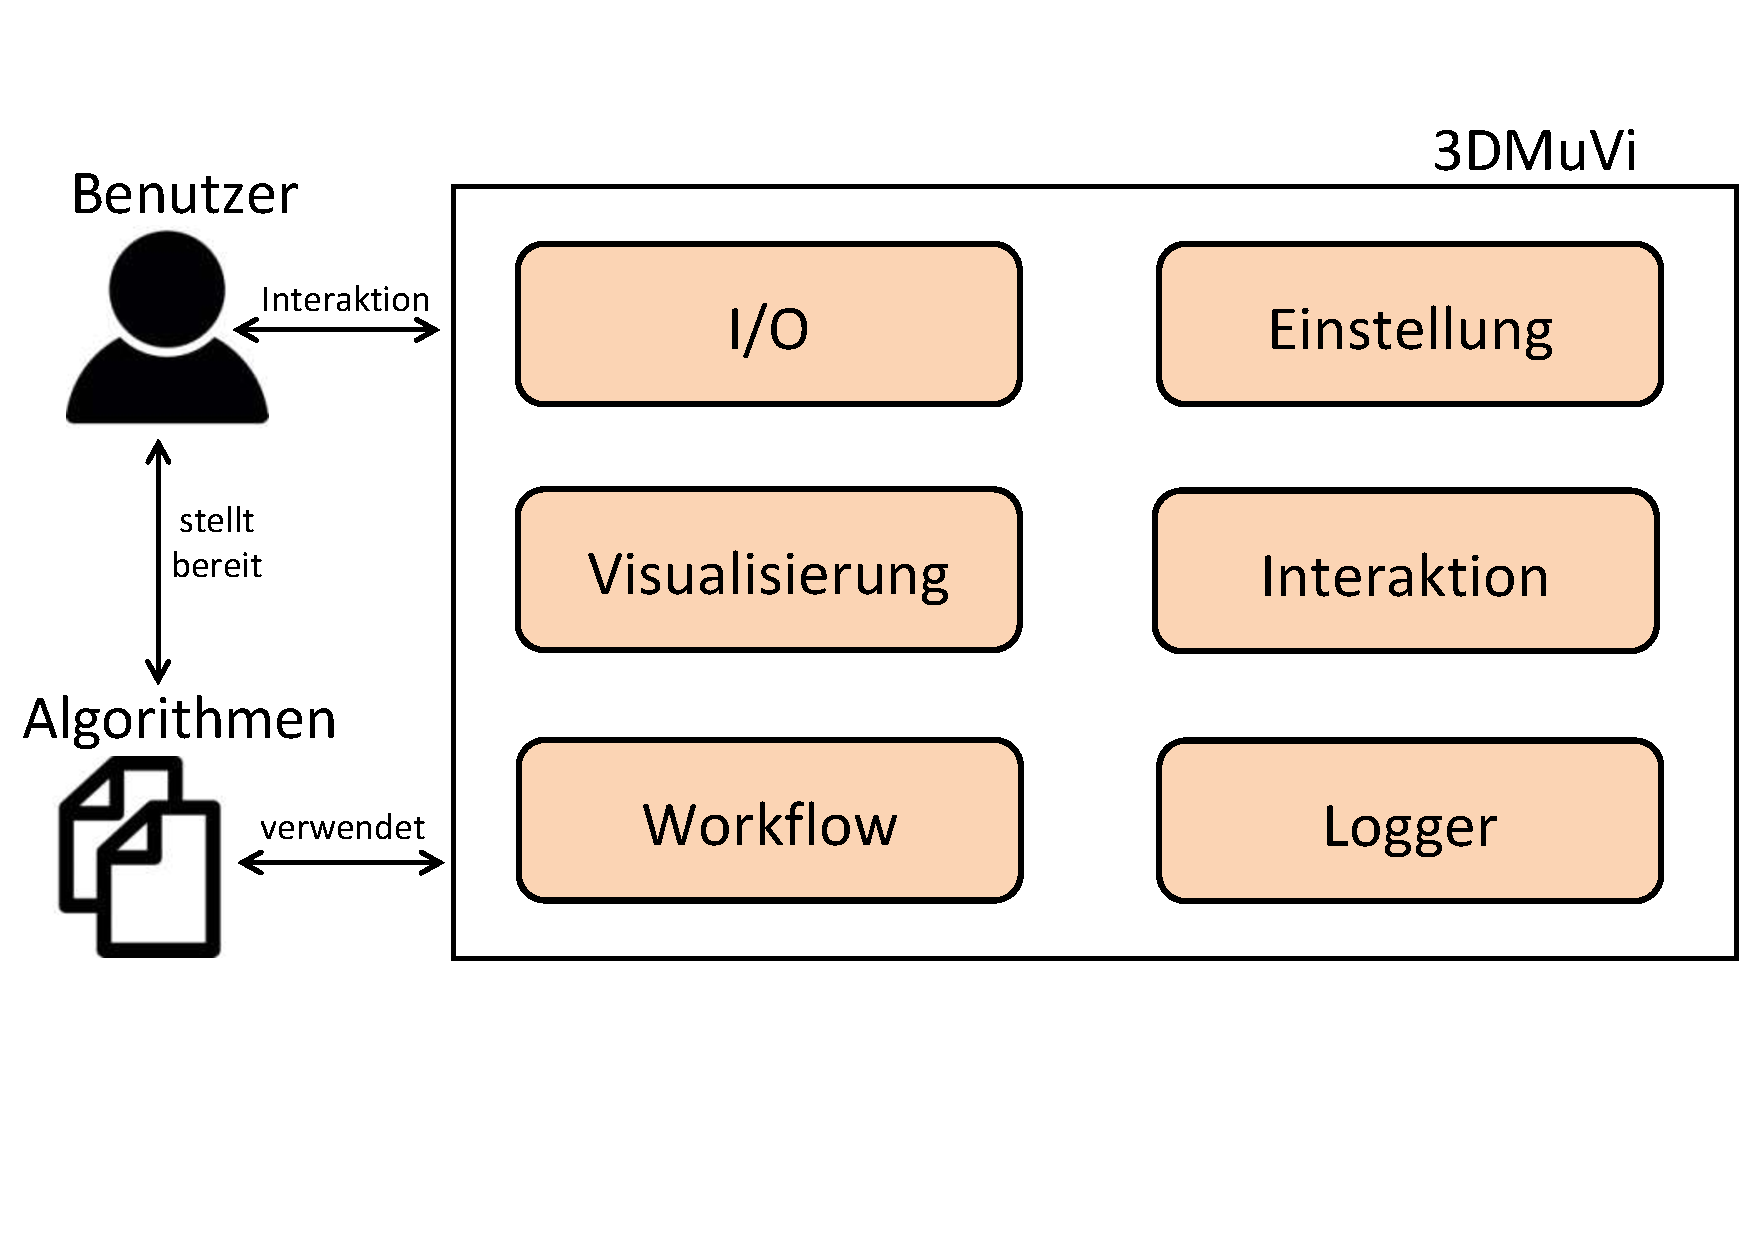
\includegraphics[width=1\textwidth]{img/SUebersicht.pdf}

\section{Module}
Im weiteren folgt eine kurze Zusammenfassung der Module.

\subsection{Workflow}
Das Modul Workflow bietet mindestens einen Workflow an und bündelt alle workflowspezifischen
Einstellungen und Auswahlmöglichkeiten, inklusive:

\begin{itemize}
\item Workflows wie den 4-Phasen-Workflow
\item Speichern und laden von Wokflowkonfigurationen
\item Algorithmenauswahl für jede Phase 
\end{itemize}

\subsection{I/O}

Das Modul I/O bietet Funktionen für die Ein- und Ausgabedaten an, inklusive:

\begin{itemize}
\item Einlesen und übergeben von Einzelbilder
\item Speichern von (Zwischen-) Ergebnissen
\end{itemize}

\subsection{Visualisierung}
Das Modul Visualisierung bietet Anzeigen der (Zwischen-) Endergebnissen  an, inklusive:

\begin{itemize}
\item Anzeigen der Ausgabedaten der (Zwischen-) Ergebniss
\end{itemize}

\subsection{Logger}
Das Modul Logger stellt Logs bereit, inklusive:

\begin{itemize}
\item Info, Warning, Error, Debug
\item Anzeige und Abspeichern dieser Logs
\end{itemize}

\subsection{Einstellung}
Das Modul Einstellungen behandelt (globale) lokale Einstellungen, inklusive:

\begin{itemize}
\item Speichern und Laden von Einstellungen einzelner Verfahren
\end{itemize}

\subsection{Interaktion}
Das Modul Interaktion behandelt Benutzereingaben innerhalb des Programms, inklusive:

\begin{itemize}
\item Starten und Stoppen, Arbeitsindikator 
\item optional, Manipulation der Ausgangsdaten der (Zwischen-) Ergebnisse
\end{itemize}

\section{Produktdaten}
Im folgenden werden alle Daten gelistet, welche abgespeichert werden.
\subsection{Daten der obligatorischen Funktionen}
\begin{enumerate}[align=left,leftmargin=4em, label={\textbf{\textbackslash PD10\arabic*0\textbackslash}} ]
	\item Zwischenergebnisse
	\item Endergebnis
	\item Parameter der einzelnen Algorithmen
\end{enumerate}
\subsection{Daten der optionalen Funktionen}
\begin{enumerate}[align=left,leftmargin=4em, label={\textbf{\textbackslash PD20\arabic*0\textbackslash}} ]
	\item Globale Einstellungen
	\item Konfiguration des Workflows
	\item Speichern weiterer Workflows
\end{enumerate}	

\section{Schnittstellen}
Hier werden die vom Programm bereitgestellten Schnittstellen beschrieben
\begin{enumerate}[ align=left, label={\textbf{\textbackslash S1\arabic*0\textbackslash}}]
\item (Funktionale-) Schnittstellen zum Aufrufen und Datenaustausch der Algorithmen
\item  Schnittstelle zum Einstellen der Algorithmen
Angabe der Config Datei und direkte Angabe eines Parameter-Trees
\end{enumerate}
\newpage 
\section{Datenflussübersicht}

Dieses Diagramm stellt eine Grobübersicht über den Datenfluss zwischen den einzelnen Modulen dar.
Diese sind nur als grobe Orientierung anzusehen und werden im Entwurf und in der Implementierung möglicherweise auf andere Weise umgesetzt.
\begin{normalsize}

\end{normalsize}
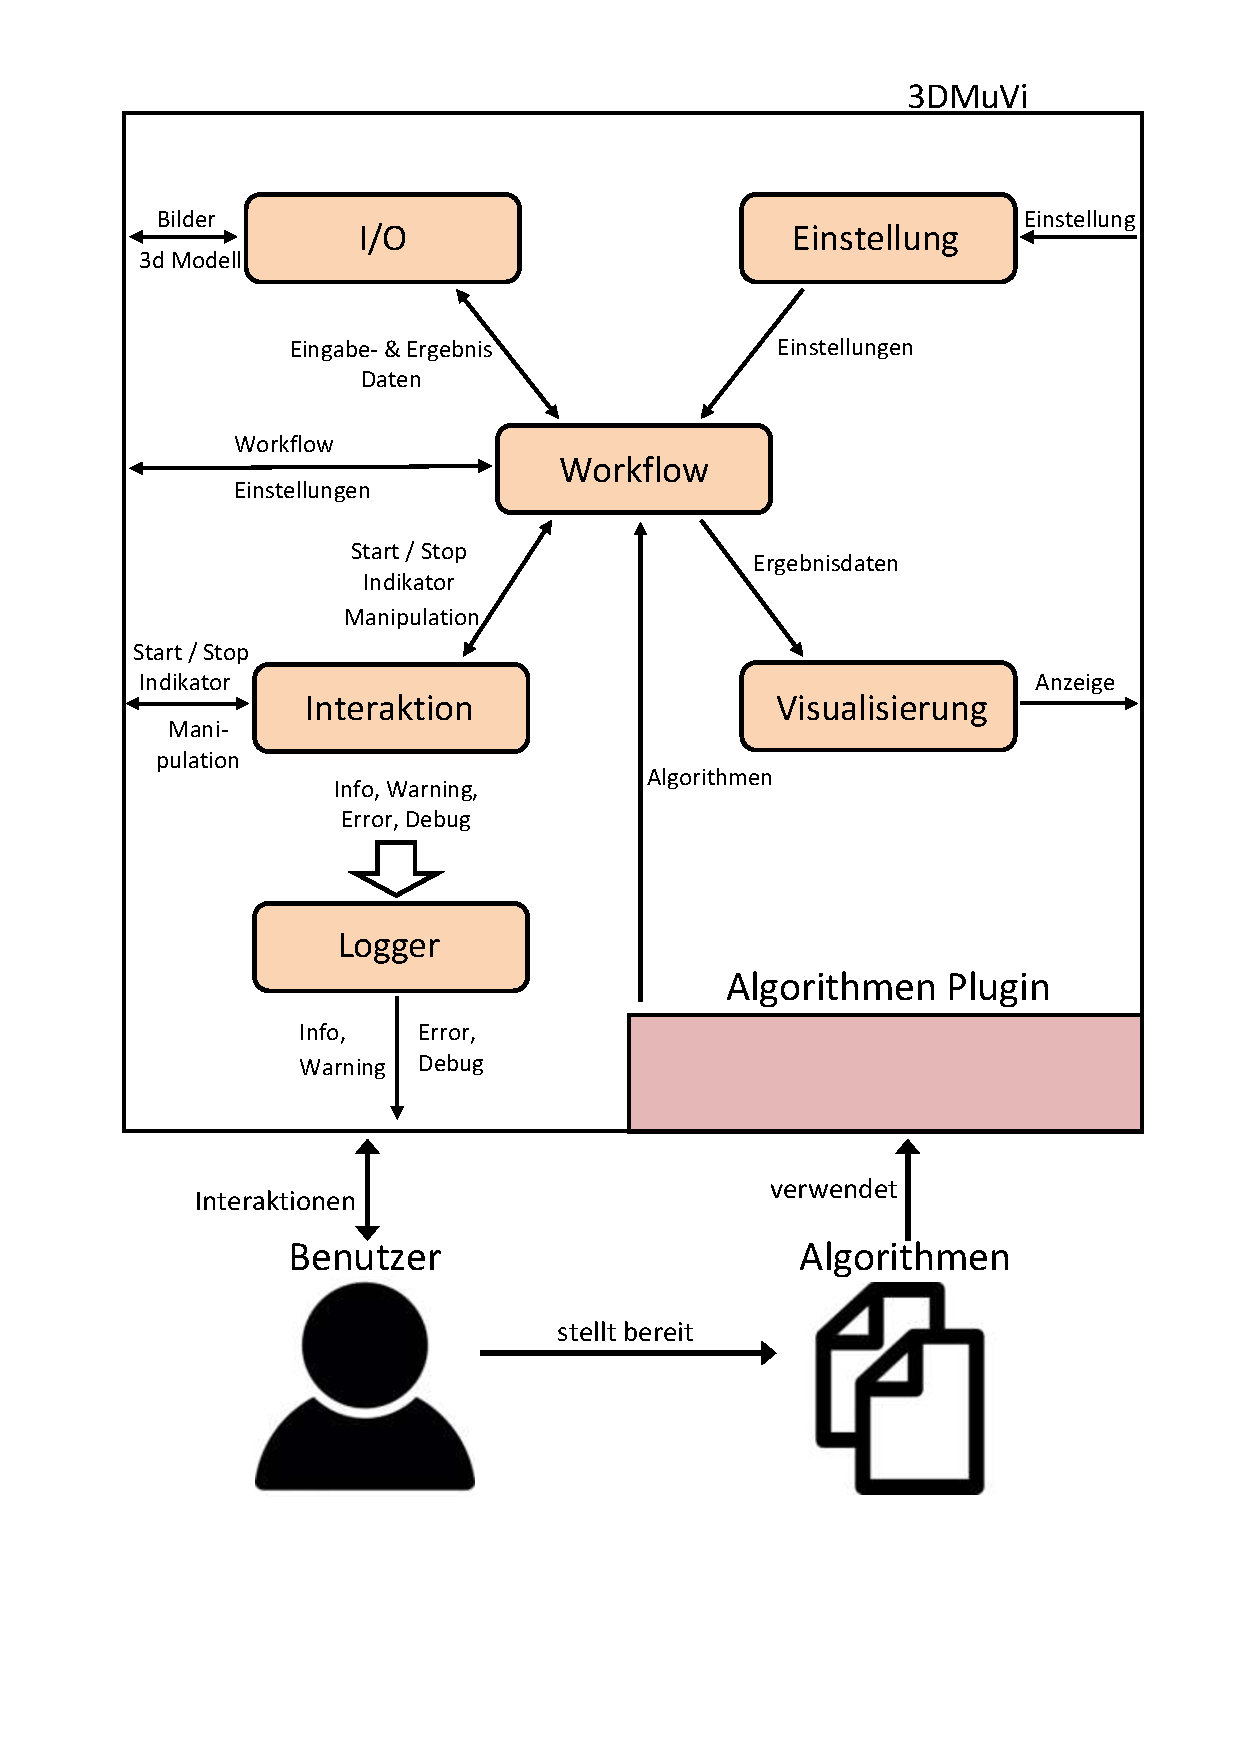
\includegraphics[width=0.87\textwidth]{img/Datenflussuebersicht.pdf} 
\newpage
 
\section{Anwendugsfälle}

\subsection{Anwendugsfall: Rekonstruktion aus unzusammenhängenden Einzelbilder}

\textbf{Gegeben:}\newline
Vielzahl an Einzelbilder einer Szene die nicht von der selben Kamera oder Position aufgenommen wurden.\newline
\textbf{Ziel:}\newline
Rekonstruktion der Szene oder eines einzelnen Objektes.\newline
\textbf{Vorgehen:}
\begin{enumerate}
\item Feature Detektor: In den Bildern wird automatisch nach „markanten“ Punkten gesucht, die hohen Wiedererkennungswert haben.\item Feature Matching: Die gefundenen „markanten Punkte“ in zwei Bildern werden verglichen und einander zugeordnet.\item Posenschätzung: Aus den Punktzuordnungen von zwei oder mehr Bildern werden die Positionen der Kameras ermittelt, von denen aus die Bilder aufgenommen wurden.\item Tiefenschätzung: Mit Hilfe der Kamerapositionen werden die Tiefen in den Bildern trianguliert. Dadurch werden die Entfernungen der Objekte auf den Bildern bestimmt.\item Modellerzeugung: Die Einzelansichten werden zu einem kompletten 3D Modell zusammengesetzt.
\end{enumerate}
\textbf{Stellschrauben:}
\begin{enumerate}
\item Der Feature Detektor kann ausgewechselt werden (z. B. SIFT oder SURF)\item Das Feature Matching kann auf verschiedene Arten durchgeführt werden (z. B. RANSAC oder MLESAC, jeweils mit verschiedener Initialisierungen)
\end{enumerate}

 
\subsection{Anwendugsfall: Structure-from-Motion (SfM)}

\textbf{Gegeben:}\newline
Videosequenz einer Szene, mit eigenbewegung der Kamera.\newline
\textbf{Ziel:}\newline
Rekonstruktion der Szene oder eines einzelnen Objektes.\newline Structure-from-Motion (SfM) ist ein Verfahren zur 3D-Rekonstruktion mit nur einer Kamera. Dabei wird bei SfM das 3D-Modell aus einem Video, also einer Reihe von Einzelbildern rekonstruiert. Dabei ist es wichtig, dass das Video nicht von einer statischen Position aus aufgenommen wird, vielmehr sollte die Kamera sich dabei mit Blick auf die zu rekonstruierende Szene bewegen. Bei der Rekonstruktion mittels SfM werden zwei oder mehr Einzelbilder der Eingangssequenz herangezogen, für die angenommen wird, dass sie dieselbe Szene aus verschiedenen Blickrichtungen betrachten und die Szene zwischen den Einzelbildern statisch (unverändert) geblieben ist.\newline
\textbf{Vorgehen:}
\begin{enumerate}
\item Feature Detection: Ermitteln leicht verfolgbarer markanter Bildpunkte\item Feature Tracking: Verfolgen der markanten Bildpunkte\item Posenschätzung: Bestimmen der Aufnahmepunkte, Verfolgen der Kamerafahrt\item Tiefenschätzung: Bestimmen der Tiefe mit lokalen Optimierungsverfahren\item Modellerzeugung: Die Einzelansichten werden zu einem kompletten 3D Modell zusammengesetzt
\end{enumerate}

\section{Typische Nutzungsabläufe}
In diesem Abschnitt werden typische Abläufe von Aktionen dargestellt, die ein Anwender mit der Software durchführt. Jeder Ablauf wird mit Hilfe eines Sequenzdiagramms visualisiert. Die Diagramme stellen nur eine Übersicht auf Modulebene dar, speziellere und ggf. angepasste Sequenzdiagramme sind dem Entwurfsdokument zu entnehmen.

\subsection{Erzeugung eines 3D-Modells}
\textbf{Vorbedingung:} Bilder des Modells wurden erstellt. \newline
\textbf{Ergebnis:} Fertiges 3D-Modell liegt zur weiteren Verarbeitung in anderer Software vor. \newline
Der Nutzer führt folgende Schritte aus (Schritte \ref{TN3DModellBilderauswahl} bis \ref{TN3DModellSpeichern} werden in 3D-MuVi ausgeführt):
\begin{enumerate}
	\item 3D-MuVi wird gestartet.
	\item \label{TN3DModellBilderauswahl} Bilder werden ausgewählt.
	\item Algorithmen für die folgenden Verarbeitungsschritte werden jeweils nacheinander ausgewählt:
	\begin{itemize}
		\item Feature Extraktion / Matching
		\item Posenschätzung
		\item Tiefenschätzung
		\item 3D Fusion
	\end{itemize}
	\item Button zum Starten der Verarbeitung wird gedrückt.
	\item \label{TN3DModellSpeichern} Ergebnisdaten werden abgespeichert.
	\item Kopieren des 3D-Modells aus dem Verzeichnisbaum der Ergebnisse an den gewünschten Ort.
\end{enumerate}
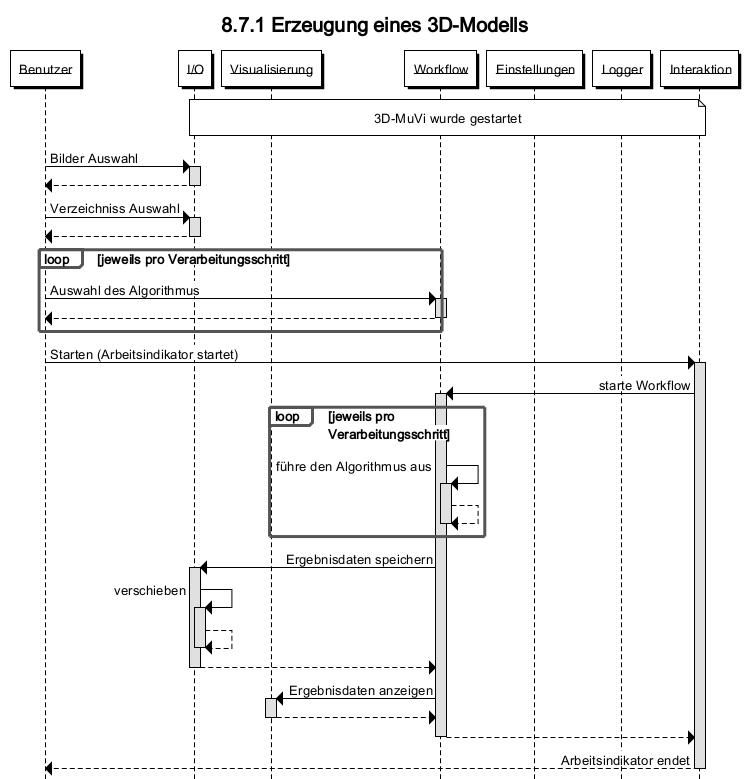
\includegraphics[width=1.05\textwidth]{img/871_Seqz.png} 

\subsection{Evaluierung von Algorithmen für Feature Extraktion / Matching}
\label{TNEvalAlgo}
\textbf{Vorbedingung:} Bilder eines Modells wurden erstellt. \newline
\textbf{Ergebnis:} Der Nutzer kann anhand der visuellen Betrachtung der Resultate einschätzen, welcher der beiden getesteten Algorithmen sich für die gewählten Bilder besser eignet. \newline
Der Nutzer führt folgende Schritte aus (Alle Schritte ab \ref{TNEvalAlgoBilderAuswahl} werden in 3D-MuVi ausgeführt):
\begin{enumerate}
	\item 3D-MuVi wird gestartet.
	\item \label{TNEvalAlgoBilderAuswahl} Bilder werden ausgewählt.
	\item Algorithmen für die folgenden Verarbeitungsschritte werden jeweils nacheinander ausgewählt:
	\begin{itemize}
		\item Feature Extraktion / Matching
		\item Posenschätzung
		\item Tiefenschätzung
		\item 3D Fusion
	\end{itemize}
	\item Button zum Starten der Verarbeitung wird gedrückt.
	\item Betrachtung der Ergebnisse.
	\item Anderer Algorithmus für den Verarbeitungsschritt Feature Extraktion / Matching wird ausgewählt.
	\item Button zum Starten der Verarbeitung wird gedrückt.
	\item Erneute Betrachtung der Ergebnisse.
\end{enumerate}
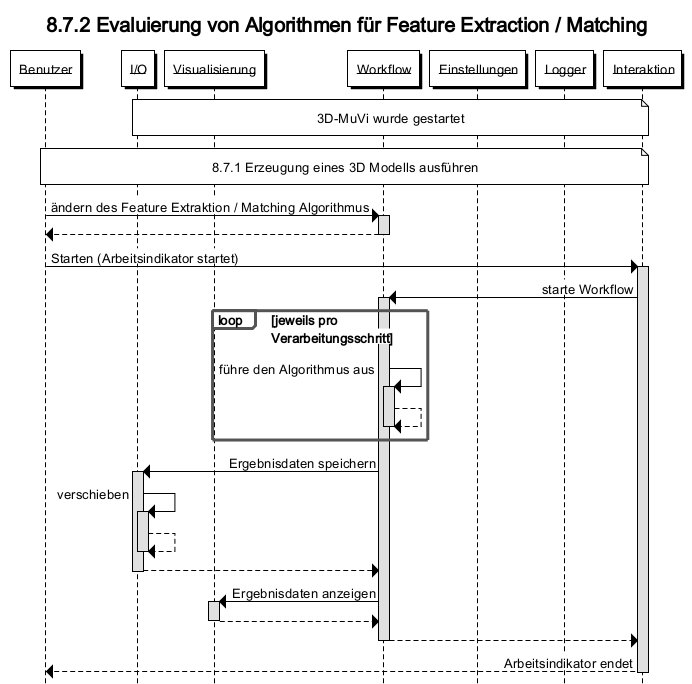
\includegraphics[width=1.05\textwidth]{img/872_Seqz.png}

\subsection{Überprüfen des Logs von Algorithmen}
\textbf{Vorbedingung:} Bilder eines Modells wurden erstellt. \newline
\textbf{Ergebnis:} Der Nutzer kann anhand der Meldungen im Log die Eignung der gewählten Algorithmen für die Bilder einschätzen und Verbesserungen an den Algorithmen vornehmen. \newline
Der Nutzer führt folgende Schritte aus (Schritte \ref{TNLogBilderAuswahl} bis \ref{TNLogSuchen} werden in 3D-MuVi ausgeführt):
\begin{enumerate}
	\item 3D-MuVi wird gestartet.
	\item \label{TNLogBilderAuswahl} Bilder werden ausgewählt.
	\item Algorithmen für die folgenden Verarbeitungsschritte werden jeweils nacheinander ausgewählt:
	\begin{itemize}
		\item Feature Extraktion / Matching
		\item Posenschätzung
		\item Tiefenschätzung
		\item 3D Fusion
	\end{itemize}
	\item Button zum Starten der Verarbeitung wird gedrückt.
	\item Alle Arten von Meldungen im Log werden eingeblendet.
	\item \label{TNLogSuchen} Auffälligkeiten in den Meldungen des Logs werden gesucht.
	\item Algorithmen werden bei Bedarf überarbeitet.
\end{enumerate}
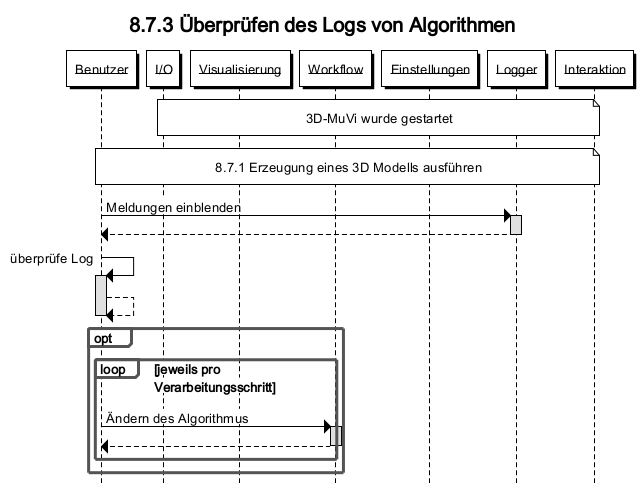
\includegraphics[width=1.05\textwidth]{img/873_Seqz.png}

\section{Typische Nutzungsabläufe mit optionalen Funktionen}

Dieser Abschnitt stellt beispielhaft typische Nutzungsabläufe dar, die möglich sind, wenn bestimmte optionale Funktionen umgesetzt sind.

\subsection{Evaluierung eines Workflows nach Entfernung eines Features in den Zwischenergebnissen}
Dieser Nutzungsablauf ist eine Erweiterung von \ref{TNEvalAlgo}. Sinn der Erweiterung ist es, dem Nutzer die Möglichkeit zu geben, das Entfernen einzelner Features zu testen, bevor er den Algorithmus entsprechend anpasst. Als optionale Funktion muss das Löschen einzelner Features in den Zwischenergebnissen und das Starten ab einem bestimmten Schritt implementiert sein. \newline
\textbf{Vorbedingung:} Bilder eines Modells wurden erstellt. \newline
\textbf{Ergebnis:} Der Nutzer kann anhand der visuellen Betrachtung der Resultate einschätzen, ob das Entfernen des Features das Endergebnis verbessert oder verschlechtert. Auf dieser Grundlage kann er über weitere Anpassungen an dem gewählten Algorithmus für die Feature Extraktion nachdenken. \newline
Der Nutzer führt folgende Schritte aus (Alle Schritte ab \ref{TNOFeatureEntfBilderAuswahl} werden in 3D-MuVi ausgeführt):
\begin{enumerate}
	\item 3D-MuVi wird gestartet.
	\item \label{TNOFeatureEntfBilderAuswahl} Bilder werden ausgewählt.
	\item Algorithmen für die folgenden Verarbeitungsschritte werden jeweils nacheinander ausgewählt:
	\begin{itemize}
		\item Feature Extraktion / Matching
		\item Posenschätzung
		\item Tiefenschätzung
		\item 3D Fusion
	\end{itemize}
	\item Button zum Starten der Verarbeitung wird gedrückt.
	\item Betrachtung der Ergebnisse.
	\item In den Ergebnissen der Feature Extraktion wird ein Feature entfernt.
	\item Button zum Starten der Verarbeitung ab dem Schritt Posenschätzung wird gedrückt.
	\item Erneute Betrachtung der Ergebnisse.
\end{enumerate}
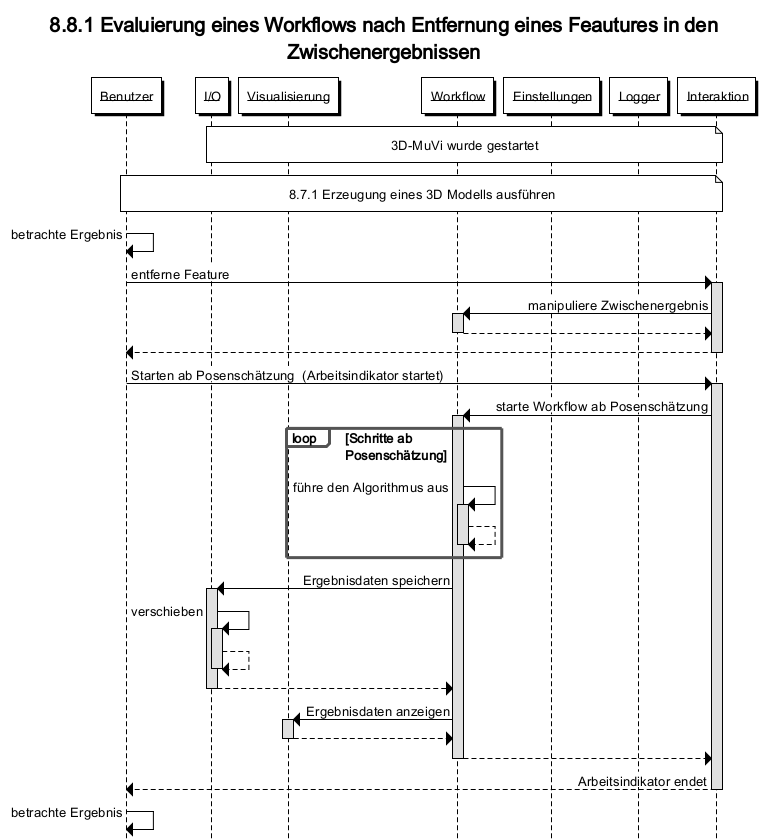
\includegraphics[width=1.05\textwidth]{img/881_Seqz.png}

\subsection{Evaluierung von Algorithmen für Feature Extraktion / Matching auf mehreren Datensätzen}
Dieser Nutzungsablauf ist eine Erweiterung von \ref{TNEvalAlgo}. Sinn der Erweiterung ist es, dem Nutzer die Möglichkeit zu geben, Workflows schnell auf mehreren Sätzen von Bildern zu evaluieren. Als optionale Funktion muss das Erstellen und Auswählen mehrerer Datensätze umgesetzt sein.\newline
\textbf{Vorbedingung:} Bilder zweier Modelle wurden erstellt (nachfolgend als Modell1 und Modell2 bezeichnet). \newline
\textbf{Ergebnis:} Der Nutzer kann anhand der visuellen Betrachtung der Resultate einschätzen, welcher der beiden getesteten Algorithmen sich für die gewählten Bilder von Modell1 bzw. Modell2 besser eignet. \newline
Der Nutzer führt folgende Schritte aus (Alle Schritte ab \ref{TNOEvalAlgoBilderAuswahl1} werden in 3D-MuVi ausgeführt):
\begin{enumerate}
	\item 3D-MuVi wird gestartet.
	\item \label{TNOEvalAlgoBilderAuswahl1} Bilder von Modell1 werden ausgewählt.
	\item Algorithmen für die folgenden Verarbeitungsschritte werden jeweils nacheinander ausgewählt:
	\begin{itemize}
		\item Feature Extraktion / Matching
		\item Posenschätzung
		\item Tiefenschätzung
		\item 3D Fusion
	\end{itemize}
	\item Button zum Starten der Verarbeitung wird gedrückt.
	\item Betrachtung der Ergebnisse.
	\item Neuer Datensatz für Modell2 wird erstellt und ausgewählt.
	\item Bilder von Modell2 werden ausgewählt.
	\item Button zum Starten der Verarbeitung wird gedrückt.
	\item Betrachtung der Ergebnisse.
	\item Anderer Algorithmus für den Verarbeitungsschritt Feature Extraktion / Matching wird ausgewählt.
	\item Button zum Starten der Verarbeitung wird gedrückt.
	\item Betrachtung der Ergebnisse.
	\item Datensatz von Modell1 wird gewählt.
	\item Betrachtung der Ergebnisse.
\end{enumerate}
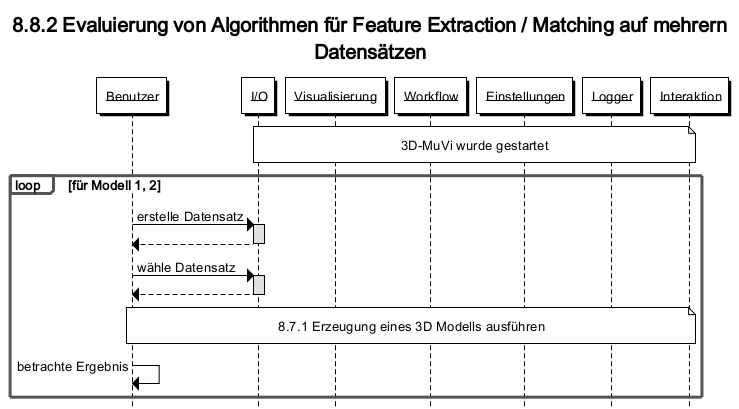
\includegraphics[width=1.05\textwidth]{img/882_Seqz.png}
%\label{ch:usecases}
%In diesem Abschnitt werden typische Abläufe von Aktionen dargestellt, die ein Anwender mit der Software durchführt.
%\subsection{Laden von Einzelbildern}
%\label{usecase:1}
%\usecase{1}
%\subsection{Auswählen von Algorithmen}
%\label{usecase:2}
%\usecase{2}
%\subsection{Ändern von Einstellungen}
%\label{usecase:3}
%\usecase{3}
%\subsection{Speichern der Einstellungen}
%\label{usecase:4}
%\usecase{4}
%\subsection{Laden von Einstellungen}
%\label{usecase:5}
%\usecase{5}
%\subsection{Öffnen der Hilfe}
%\label{usecase:6}
%\usecase{6}
%\subsection{Filtern der Logs}
%\label{usecase:7}
%\usecase{7}
%\subsection{Ausführen von Algorithmen}
%\label{usecase:8}
%\usecase{8}
%\subsection{Unterbrechen der Verarbeitung}
%\label{usecase:9}
%\usecase{9}
%\subsection{Vorschau der Ergebnisse}
%\label{usecase:10}
%\usecase{10}
%
%
%\iffalse
%\fi

